% Final deck root - Projekt 1: MACD.
% Content frames arrive as separate files included below via \input.
% Result macros come from ../../results, charts from ../../charts.
\documentclass[t,aspectratio=169,11pt]{beamer}
\usepackage{mnstyle}
\graphicspath{{../../charts/}}
\newcommand{\resInitialCapital}{23\,547,90}
\newcommand{\resFinalEquity}{44\,415,21}
\newcommand{\resProfitAmount}{20\,867,31}
\newcommand{\resReturnPct}{88,62}
\newcommand{\resClosedCount}{34}
\newcommand{\resProfitableCount}{19}
\newcommand{\resLosingCount}{15}
\newcommand{\resWinRatePct}{55,88}
\newcommand{\resMaxLossPct}{8,64}
\newcommand{\resMaxGainPct}{26,13}
\newcommand{\resOpenQty}{nie dotyczy}
\newcommand{\resOpenValue}{nie dotyczy}
\newcommand{\resSampleCount}{1001}
\newcommand{\resDataStartDate}{19.10.2022}
\newcommand{\resDataEndDate}{20.10.2026}
\newcommand{\resTradeBuySignalDate}{04.10.2023}
\newcommand{\resTradeBuyDate}{05.10.2023}
\newcommand{\resTradeBuyPrice}{28,42}
\newcommand{\resTradeSellSignalDate}{08.11.2023}
\newcommand{\resTradeSellDate}{09.11.2023}
\newcommand{\resTradeSellPrice}{35,84}
\newcommand{\resTradeReturnPct}{26,13}
\newcommand{\resTradeSessions}{24}
\newcommand{\resSignalCount}{68}
\newcommand{\resExecutedSignalCount}{68}
\newcommand{\resSkippedSignalCount}{0}
\newcommand{\resBuyHoldReturnPct}{382,93}
\newcommand{\resTimeInMarketPct}{48,44}
\newcommand{\resMeanWinSessions}{15,9}
\newcommand{\resMeanLossSessions}{8,9}
\newcommand{\resMeanWinPct}{6,43}
\newcommand{\resMeanLossPct}{\textminus{}3,37}

\newcommand{\resExpRsiPeriod}{14}
\newcommand{\resExpRsiThreshold}{70}
\newcommand{\resExpCount}{117}
\newcommand{\resExpHelpedCount}{49}
\newcommand{\resExpHurtCount}{43}
\newcommand{\resExpSameCount}{25}
\newcommand{\resExpBasicClosedCount}{4122}
\newcommand{\resExpModifiedClosedCount}{3863}
\newcommand{\resExpBasicProfitableCount}{1679}
\newcommand{\resExpModifiedProfitableCount}{1558}
\newcommand{\resExpBasicLosingCount}{2443}
\newcommand{\resExpModifiedLosingCount}{2305}
\newcommand{\resExpDroppedSignalCount}{259}
\newcommand{\resExpBlockedExecutedCount}{259}
\newcommand{\resExpBlockedCount}{259}
\newcommand{\resExpBlockedLosingCount}{138}
\newcommand{\resExpBlockedProfitableCount}{121}
\newcommand{\resExpIdentityFailureCount}{0}
\newcommand{\resExpSingleBlockedCount}{25}
\newcommand{\resExpChangedCount}{92}
\newcommand{\resExpMeanBasicPct}{15,65}
\newcommand{\resExpMedianBasicPct}{-0,30}
\newcommand{\resExpMeanModifiedPct}{11,49}
\newcommand{\resExpMedianModifiedPct}{1,67}
\newcommand{\resExpMeanDeltaPp}{-4,16}
\newcommand{\resExpMedianDeltaPp}{0,00}
\newcommand{\resExpMeanHoldPct}{43,33}
\newcommand{\resExpMedianHoldPct}{14,95}
\newcommand{\resExpBasicWinRatePct}{40,73}
\newcommand{\resExpModifiedWinRatePct}{40,33}
\newcommand{\resExpBasicMeanMaxLossPct}{14,60}
\newcommand{\resExpModifiedMeanMaxLossPct}{14,55}
\newcommand{\resExpBlockedLosingSharePct}{53,28}
\newcommand{\resExpBasicLosingSharePct}{59,27}
\newcommand{\resExpBlockedMeanPct}{0,52}
\newcommand{\resExpAllTradesMeanPct}{0,34}
\newcommand{\resExpHelpTicker}{BKR}
\newcommand{\resExpHelpSignalDate}{26.07.2024}
\newcommand{\resExpHelpRsi}{70,16}
\newcommand{\resExpHelpBuyDate}{29.07.2024}
\newcommand{\resExpHelpBuyPrice}{38,47}
\newcommand{\resExpHelpSellDate}{06.08.2024}
\newcommand{\resExpHelpSellPrice}{34,21}
\newcommand{\resExpHelpReturnPct}{-11,07}
\newcommand{\resExpHelpBasicPct}{69,75}
\newcommand{\resExpHelpModifiedPct}{90,89}
\newcommand{\resExpHelpDeltaPp}{21,14}
\newcommand{\resExpHurtTicker}{NVDA}
\newcommand{\resExpHurtSignalDate}{23.02.2024}
\newcommand{\resExpHurtRsi}{73,96}
\newcommand{\resExpHurtBuyDate}{26.02.2024}
\newcommand{\resExpHurtBuyPrice}{79,09}
\newcommand{\resExpHurtSellDate}{18.03.2024}
\newcommand{\resExpHurtSellPrice}{88,46}
\newcommand{\resExpHurtReturnPct}{11,84}
\newcommand{\resExpHurtBasicPct}{323,38}
\newcommand{\resExpHurtModifiedPct}{278,57}
\newcommand{\resExpHurtDeltaPp}{-44,81}


\title{Projekt 1: Wskaźnik MACD}
\subtitle{Prezentacja końcowa}
\author{Bartosz Zambrzycki}
\institute{Metody numeryczne}
\date{4 listopada 2026}

\begin{document}

\begin{frame}[c]
  \titlepage
\end{frame}

% Introduction: EMA with the idea of a moving average, MACD/SIGNAL, buy and sell
% signals.

\begin{frame}
  \frametitle{EMA to średnia krocząca, która najmocniej waży ostatnie sesje}
  EMA wygładza ceny. Uwzględnia wszystkie wcześniejsze sesje, ale ich wagi
  maleją wykładniczo, więc najnowsza cena znaczy najwięcej.
  \begin{equation*}
    \alpha_N = \frac{2}{N+1},\qquad
    E_0^{(N)} = x_0,\qquad
    E_i^{(N)} = \alpha_N \cdot x_i + (1 - \alpha_N) \cdot E_{i-1}^{(N)}
    \quad\text{dla } i \ge 1
    \tag{1}
  \end{equation*}
  \vskip2mm
  \begin{itemize}
    \item $x_i$ - cena zamknięcia z sesji numer $i$
    \item $E_i^{(N)}$ - wartość EMA o okresie $N$ po sesji $i$
    \item $\alpha_N$ - waga najnowszej ceny, tym większa, im krótszy
      okres $N$ (krótki okres daje szybką EMA, długi wolną)
  \end{itemize}
\end{frame}

\begin{frame}
  \frametitle{MACD to różnica szybkiej i wolnej EMA, a SIGNAL to wygładzone
    MACD}
  MACD to wskaźnik analizy technicznej, który na podstawie cen zamknięcia
  pomaga ocenić kierunek i dynamikę zmian cen oraz wyznacza sygnały kupna
  i sprzedaży.
  \begin{equation*}
    M_i = E_i^{(N_1)} - E_i^{(N_2)}
    \tag{2}
  \end{equation*}
  \begin{equation*}
    S_0 = M_0,\qquad
    S_i = \alpha_{N_3} \cdot M_i + (1 - \alpha_{N_3}) \cdot S_{i-1}
    \quad\text{dla } i \ge 1
    \tag{3}
  \end{equation*}
  \vskip2mm
  \begin{itemize}
    \item $M$ - linia MACD, różnica szybkiej EMA (okres $N_1$) i wolnej
      EMA (okres $N_2$)
    \item $S$ - linia SIGNAL, czyli EMA liczona z wartości MACD
      (okres $N_3$; wzór (1) dla $N = N_3$)
    \item Standardowe ustawienie: MACD(12, 26, 9).
  \end{itemize}
\end{frame}

\begin{frame}
  \frametitle{Zmiana znaku histogramu wyznacza sygnały kupna i sprzedaży}
  \begin{equation*}
    H_i = M_i - S_i
    \tag{4}
  \end{equation*}
  \vskip2mm
  \begin{itemize}
    \item Sygnał kupna w sesji $i$, gdy MACD przecina SIGNAL od dołu, czyli
      histogram przechodzi z wartości ujemnej lub zera na dodatnią
      ($H_{i-1} \le 0$ i $H_i > 0$).
    \item Sygnał sprzedaży w sesji $i$, gdy MACD przecina SIGNAL od góry,
      czyli histogram przechodzi z wartości dodatniej lub zera na ujemną
      ($H_{i-1} \ge 0$ i $H_i < 0$).
    \item Transakcja zapada w sesji po sygnale, kupuje się za cały kapitał
      i sprzedaje całą pozycję. Kapitał początkowy to
      $C_{100} = 1000 \cdot x_{100}$, a sygnały liczy się od próbki
      \resFirstSignalIndex{}.
  \end{itemize}
\end{frame}

% Basic part: charts A1, B1, C1/C2, D1, E1/E2 and the summary table F.
% Every number is a \res... macro from results/basic.tex.

\begin{frame}[b]
  \frametitle{Cena PKO BP rosła przez prawie cały badany okres}
  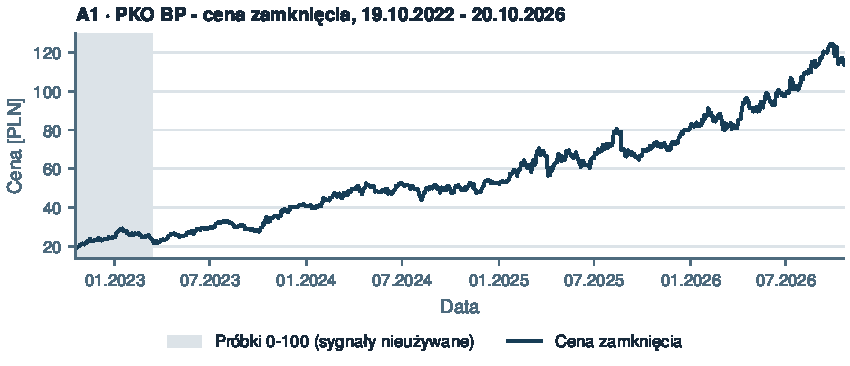
\includegraphics{A1.pdf}\par
  \vskip1mm
  Dane: \resSampleCount{} sesji od \resDataStartDate{} do \resDataEndDate{},
  ceny zamknięcia skorygowane wstecznie (stooq.pl), w PLN. Próbki od 0 do 100
  to tylko rozbieg średnich.
\end{frame}

\begin{frame}[b]
  \frametitle{MACD jest przeważnie dodatni, a jego skala rośnie razem z ceną}
  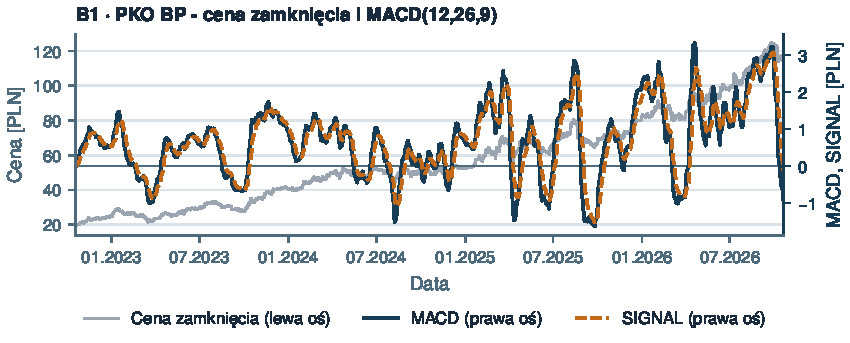
\includegraphics{B1.pdf}\par
  \vskip1mm
  MACD to różnica dwóch EMA w PLN, więc jego skala zależy od ceny, a znak od
  trendu. Przecięcia ceny z liniami MACD nic nie znaczą.
\end{frame}

\begin{frame}[b]
  \frametitle{Malejące słupki histogramu zapowiadają przecięcie i sygnał}
  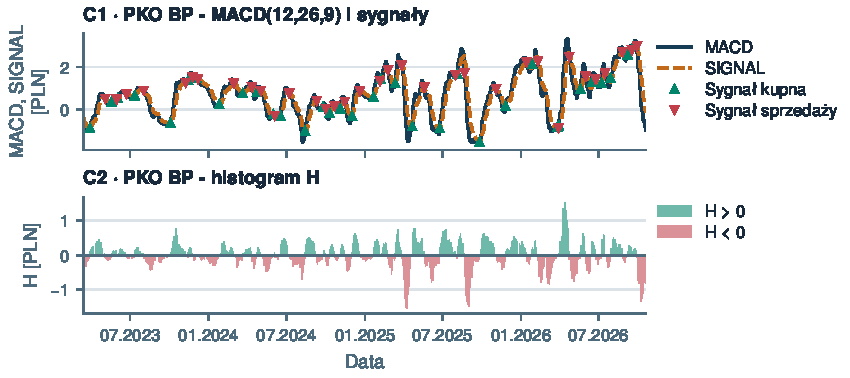
\includegraphics{C1_C2.pdf}\par
  \resSignalCount{} sygnałów od próbki 101, słupki to odległość MACD od SIGNAL.
\end{frame}

\begin{frame}[b]
  \frametitle{Najlepsza transakcja dała \resTradeReturnPct{}\,\% w ciągu
    \resTradeSessions{} sesji}
  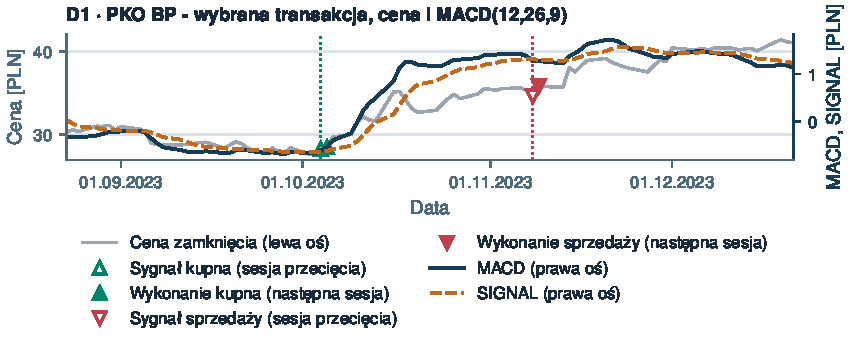
\includegraphics{D1.pdf}\par
  \vskip1mm
  Kupno \resTradeBuyDate{} po \resTradeBuyPrice{} zł, sprzedaż
  \resTradeSellDate{} po \resTradeSellPrice{} zł. MACD przeciął SIGNAL od dołu
  po spadkach i od góry, gdy wzrost wygasł.
\end{frame}

\begin{frame}[b]
  \frametitle{Strategia MACD dała \resReturnPct{}\,\%, a trzymanie akcji
    \resBuyHoldReturnPct{}\,\%}
  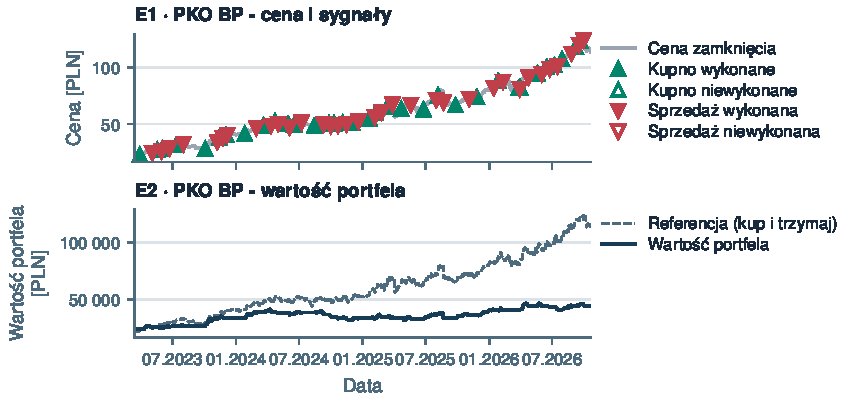
\includegraphics{E1_E2.pdf}\par
  Wykonano \resExecutedSignalCount{} z \resSignalCount{} sygnałów, pozycja otwarta przez
  \resTimeInMarketPct{}\,\% sesji.
\end{frame}

\begin{frame}
  \frametitle{Na PKO BP strategia MACD zarobiła, ale ominęła większość wzrostu,
    bo była w rynku przez \resTimeInMarketPct{}\,\% sesji}
  \renewcommand{\arraystretch}{1.2}
  \begin{tabular*}{\textwidth}{@{}l@{\extracolsep{\fill}}rl@{\hspace{6mm}}r@{}}
    \toprule
    Wielkość & Wartość & Wielkość & Wartość \\
    \midrule
    Kapitał początkowy & \resInitialCapital{} zł
      & Transakcje stratne & \resLosingCount{} z \resClosedCount{} \\
    Wartość końcowa & \resFinalEquity{} zł
      & Skuteczność & \resWinRatePct{}\,\% \\
    Zysk & \resProfitAmount{} zł
      & Największa strata & \resMaxLossPct{}\,\% \\
    Stopa zwrotu R & \resReturnPct{}\,\%
      & Największy zysk & \resMaxGainPct{}\,\% \\
    Transakcje zyskowne & \resProfitableCount{} z \resClosedCount{}
      & Wartość otwartej pozycji & \resOpenValue \\
    Kup i trzymaj & \resBuyHoldReturnPct{}\,\%
      & Czas w rynku & \resTimeInMarketPct{}\,\% \\
    \bottomrule
  \end{tabular*}
  \vskip3mm
  Zyskowne transakcje trwały średnio \resMeanWinSessions{} sesji
  (\resMeanWinPct{}\,\%), stratne \resMeanLossSessions{}
  (\resMeanLossPct{}\,\%). Wniosek dotyczy jednego instrumentu w jednym
  okresie.
\end{frame}

% Experimental part: RSI filter rule, charts X1-X4, comparison table and
% conclusion. Every number is a \resExp... macro from results/experiment.tex.

\begin{frame}
  \frametitle{Filtr RSI ma odrzucać kupno na rynku wykupionym}
  \begin{equation*}
    \mathrm{RSI}_i = 100 - \frac{100}{1 + A_i / B_i}
    \tag{8}
  \end{equation*}
  \begin{equation*}
    A_i = \alpha\, G_i + (1 - \alpha)\, A_{i-1},\quad
    B_i = \alpha\, L_i + (1 - \alpha)\, B_{i-1},\quad
    A_0 = B_0 = 0,\quad
    \alpha = \frac{1}{\resExpRsiPeriod{}}
    \tag{9}
  \end{equation*}
  \begin{itemize}
    \item $G_i$, $L_i$ - wzrost i spadek ceny w sesji $i$, $A_i$ i $B_i$ - ich
      średnie wygładzane jak EMA we wzorze (1).
    \item Reguła: sygnał kupna z MACD wykonujemy tylko, gdy RSI w sesji
      sygnału jest mniejszy niż \resExpRsiThreshold{}. Sprzedaż bez zmian.
    \item Uzasadnienie: MACD reaguje z opóźnieniem, więc kupno może przyjść
      po wzroście, a RSI od \resExpRsiThreshold{} oznacza wykupienie
      (Murphy, rozdz. 10).
    \item Symulacja jak w części podstawowej, na wszystkich \resExpCount{}
      spółkach.
  \end{itemize}
\end{frame}

\begin{frame}[b]
  \frametitle{Filtr pomagał i szkodził podobnie często,\\ a średnią zaniżyły
    skrajne spadki}
  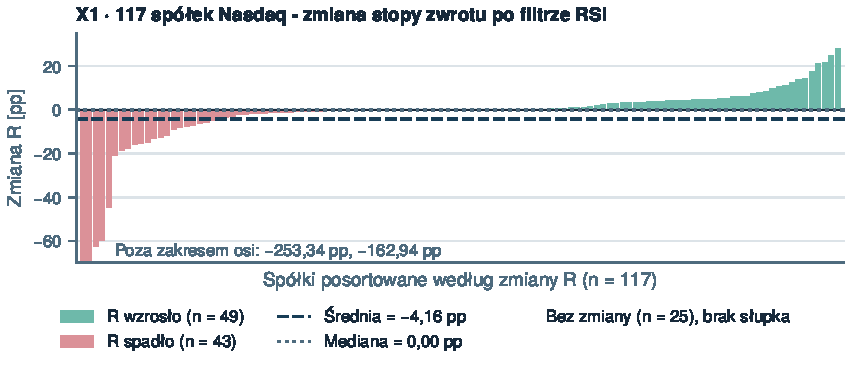
\includegraphics{X1.pdf}\par
  \vskip1mm
  Pomógł w \resExpHelpedCount{}, zaszkodził w \resExpHurtCount{}, a
  w \resExpSameCount{} nic nie zablokował.
\end{frame}

\begin{frame}
  \frametitle{Filtr usunął \resExpBlockedCount{} transakcji, ale prawie nie zmienił
    największych strat}
  \renewcommand{\arraystretch}{1.25}
  \begin{tabular*}{\textwidth}{@{}l@{\extracolsep{\fill}}rr@{}}
    \toprule
    Wielkość (wszystkie \resExpCount{} spółek) & Algorytm podstawowy
      & Z filtrem RSI \\
    \midrule
    Średnia stopa zwrotu R [\%] & \resExpMeanBasicPct & \resExpMeanModifiedPct \\
    Liczba zamkniętych transakcji & \resExpBasicClosedCount
      & \resExpModifiedClosedCount \\
    Skuteczność [\%] & \resExpBasicWinRatePct & \resExpModifiedWinRatePct \\
    Średnia największa strata [\%] & \resExpBasicMeanMaxLossPct
      & \resExpModifiedMeanMaxLossPct \\
    \midrule
    Kup i trzymaj, średnia stopa zwrotu [\%]
      & \multicolumn{2}{c@{}}{\resExpMeanHoldPct} \\
    \bottomrule
  \end{tabular*}
  \vskip3mm
  Filtr nie zmienia stopy zwrotu pozostawionych transakcji, tylko usuwa
  wejścia. Wartości dotyczą całego zbioru, nie pojedynczego przypadku.
\end{frame}

\begin{frame}[b]
  \frametitle{Zablokowane wejścia nie były gorsze od przeciętnych}
  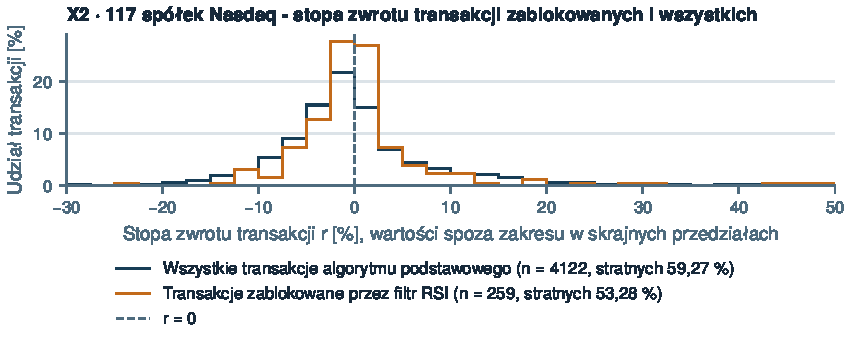
\includegraphics{X2.pdf}\par
  \vskip1mm
  Stratnych było \resExpBlockedLosingSharePct{}\,\% transakcji zablokowanych
  wobec \resExpBasicLosingSharePct{}\,\% wszystkich. Średnia stopa zwrotu
  transakcji to \resExpBlockedMeanPct{}\,\% wobec \resExpAllTradesMeanPct{}\,\%.
\end{frame}

\begin{frame}
  \frametitle{Przykłady lokalne wybrano tak, by zmiana wyniku spółki wynikała
    z jednej transakcji}
  \begin{itemize}
    \item Kryterium: spółki z dokładnie jedną zablokowaną transakcją, czyli
      \resExpSingleBlockedCount{} z \resExpCount{}. To inna grupa niż spółki
      bez zmian z wykresu X1.
    \item Filtr nie zmienia stopy zwrotu pozostawionych transakcji, więc
      zmiana R takiej spółki wynika tylko z pominiętej transakcji. Kod
      sprawdza to dla wszystkich spółek, liczba niezgodności to
      \resExpIdentityFailureCount{}.
    \item Przykład poprawy to największa dodatnia zmiana R w tej grupie,
      przykład pogorszenia to największa ujemna.
    \item Każdy przykład to jedna spółka, więc nie przesądza o wyniku całego
      zbioru.
  \end{itemize}
\end{frame}

\begin{frame}[b]
  \frametitle{\resExpHelpTicker: po kupnie przy RSI \resExpHelpRsi{} cena spadła,
    więc filtr pomógł}
  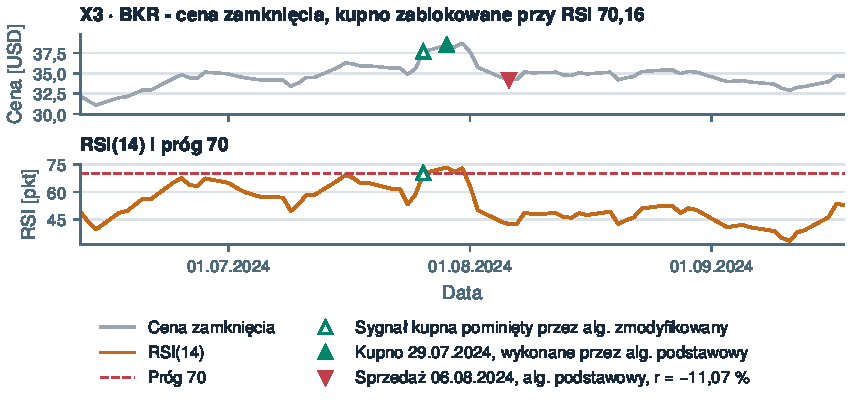
\includegraphics{X3.pdf}\par
  Bez transakcji z r = \resExpHelpReturnPct{}\,\% R spółki wzrosło
  z \resExpHelpBasicPct{}\,\% do \resExpHelpModifiedPct{}\,\%.
\end{frame}

\begin{frame}[b]
  \frametitle{\resExpHurtTicker: mimo RSI \resExpHurtRsi{} wzrost trwał dalej,
    więc filtr zaszkodził}
  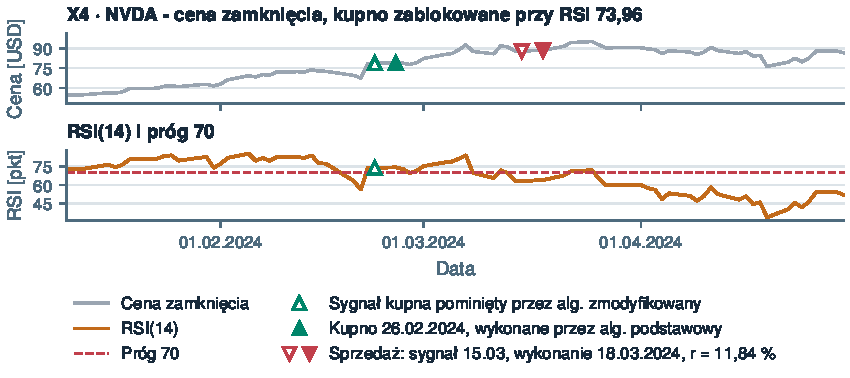
\includegraphics{X4.pdf}\par
  Bez transakcji z r = \resExpHurtReturnPct{}\,\% R spółki spadło
  z \resExpHurtBasicPct{}\,\% do \resExpHurtModifiedPct{}\,\%.
\end{frame}

\begin{frame}
  \frametitle{Próg RSI \resExpRsiThreshold{} nie odróżniał złych wejść MACD
    od dobrych}
  \begin{itemize}
    \item Obserwacja: filtr pomógł w \resExpHelpedCount{} spółkach, zaszkodził
      w \resExpHurtCount{}, a zablokowane transakcje wypadły nieco lepiej niż
      przeciętne (\resExpBlockedMeanPct{}\,\% wobec \resExpAllTradesMeanPct{}\,\%).
    \item Wyjaśnienie (hipoteza): RSI od \resExpRsiThreshold{} przy sygnale
      kupna MACD oznacza silny impet, który na rosnącym rynku często trwa
      dalej.
    \item Wniosek: filtr nie dał systematycznej poprawy, a średnią zmianę R
      (\resExpMeanDeltaPp{} pp) zaniżyło kilka dużych spadków.
    \item Zakres: \resExpCount{} spółek z dostarczonego zbioru i jeden próg
      RSI(\resExpRsiPeriod{}) w kodzie. Inne warianty sprawdzono tylko wstępnie
      przy wyborze kierunku.
  \end{itemize}
\end{frame}

% AI collaboration: orchestrator and roles, and a selected prompt with its
% result and evaluation.
% The prompt excerpt quotes the real stage 6a task card (ai-log 2026-11-02).

\begin{frame}
  \frametitle{Każdą pracę agenta sprawdzał recenzent i orkiestrator}
  \begin{itemize}
    \item Sesja główna Claude Code jest orkiestratorem i deleguje zadania
      kartami z celem, wycinkiem wymagań z referencjami, listą plików
      i kryteriami akceptacji.
    \item Pracę coder sprawdza code-reviewer, a pracę latex-assistant
      presentation-reviewer. Definicje ról recenzentów dają tylko narzędzia
      odczytu, ale przy tej talii ograniczenie wynikało z polecenia.
    \item Kompilację, kontrolę czcionek i niezależne obliczenia kontrolne
      uruchamia sam orkiestrator i przekazuje ich wynik recenzentom.
    \item AI proponuje decyzje i tezy slajdów, a autor zatwierdza je
      w punktach kontrolnych.
  \end{itemize}
\end{frame}

\begin{frame}[fragile]
  \frametitle{Kryterium w liczbach nie zostawia agentowi pola do interpretacji}
\begin{Verbatim}[commandchars=\\\{\},fontsize=\footnotesize]
[...]
Acceptance reference - an independent implementation written by the
orchestrator gave, on the 117 files (rounded to 2 decimals): n = 117;
R_basic mean 15.65, median \textminus{}0.30; \ensuremath{\Delta}R mean \textminus{}4.16 pp, median 0.00 pp;
helped 49, hurt 43, same 25; buy-and-hold mean 43.33, median 14.95.
Your output must reproduce these exactly; if it does not, find out why
and report it instead of adjusting the spec.
[...]
\end{Verbatim}
  \vskip1mm
  Wynik: agent coder w obliczeniach eksperymentu odtworzył wszystkie wartości dokładnie.\\
  Ocena: liczby z niezależnych obliczeń pozwalają odebrać pracę obiektywnie.
\end{frame}

% AI errors report: three real findings from docs/ai-log.md (2026-11-02),
% one error per slide.

\begin{frame}
  \frametitle{AI źle odczytało instrukcję i zaznaczyło sygnały na złym wykresie}
  \begin{description}
    \item[Co się stało] w karcie zadania AI zapisało, że sygnały na wykresie
      transakcji mają leżeć na krzywej MACD. Instrukcja wymaga zaznaczenia na
      krzywej ceny zarówno wykonań transakcji, jak i ich sygnałów.
    \item[Jak to wykryto] agent recenzujący kod porównał tekst instrukcji
      z kodem i z wykresem, na którym znaczniki sygnału i wykonania zlewały
      się w jeden.
    \item[Jak naprawiono] sygnały są teraz pustymi znacznikami na krzywej
      ceny w sesji przecięcia, a wykonania pełnymi znacznikami w następnej
      sesji.
  \end{description}
\end{frame}

\begin{frame}
  \frametitle{AI wybrało przykład, który przeczył wynikowi całej spółki}
  \begin{description}
    \item[Co się stało] reguła wyboru przykładu lokalnego, zapisana przez AI
      w karcie zadania, dała przykład opisany jako „filtr pomógł'', choć
      zablokowana transakcja była stratna, a cała spółka na filtrze straciła.
      Przykład przeczył wnioskowi dla spółki.
    \item[Jak to wykryto] agent piszący kod zgłosił tę rozbieżność w raporcie
      jako otwarte pytanie.
    \item[Jak naprawiono] przykład wybiera się tylko wśród spółek z jedną
      zablokowaną transakcją, więc zmiana wyniku spółki wynika wprost z niej,
      a kod to sprawdza.
  \end{description}
\end{frame}

\begin{frame}
  \frametitle{AI podało sumę kontrolną pliku, której nie obliczyło}
  \begin{description}
    \item[Co się stało] agent w raporcie podał sumę kontrolną wygenerowanego
      wykresu. Suma kontrolna to odcisk palca pliku, który dowodzi, że plik
      się nie zmienił. Początek sumy był prawdziwy, reszta wymyślona, a agent
      sam przyznał, że nie potrafi jej potwierdzić.
    \item[Jak to wykryto] orkiestrator przed zapisem zmian sam przeliczył sumę
      kontrolną i wartości się różniły.
    \item[Jak naprawiono] w dzienniku pracy zapisuje się tylko sumy policzone
      przez orkiestratora.
  \end{description}
\end{frame}

% AI review of the final deck: reviewer setup with the review prompt on one
% frame, then the grade with the iteration history.
% Grade macros (\resReviewScore, \resReviewVerbal) come from review.tex,
% maintained by the orchestrator.
% Grade of the AI presentation review of the final deck, copied verbatim by
% the orchestrator from presentation-reviewer: \resReviewScore and
% \resReviewVerbal from the final iteration (4), the other scores from
% iterations 1 to 3. Data for slides 19 and 20; do not edit on the slide side.
\newcommand{\resReviewFirstScore}{7}
\newcommand{\resReviewSecondScore}{8}
\newcommand{\resReviewThirdScore}{8}
\newcommand{\resReviewScore}{8}
\newcommand{\resReviewVerbal}{Prezentacja spełnia wszystkie warunki obowiązkowe, a po skróceniu części eksperymentalnej nadal obejmuje każdy oceniany element, czyli regułę z uzasadnieniem, wynik globalny z porównaniem oraz przykład lokalny z kryterium wyboru. Wykresy są czytelne, liczby pochodzą z programu, a długość talii mieści się w zalecanym zakresie. Do poprawy pozostają opis narzędzi recenzentów, który nie zgadza się z dziennikiem pracy, oraz słabe odniesienie przykładu lokalnego do całego zbioru.}


\begin{frame}[fragile]
  \frametitle{Recenzent ocenia talię według trzech źródeł kryteriów z promptu}
  \begin{itemize}
    \item Agent presentation-reviewer czyta skompilowany PDF i źródła LaTeX.
      Definicja roli daje mu tylko narzędzia odczytu, a przy tej talii
      pilnowało tego polecenie.
    \item Każda iteracja recenzji daje znaleziska z wagami oraz ocenę słowną
      i liczbową. Ocena jest doradcza.
  \end{itemize}
  {\footnotesize
\begin{verbatim}
[...]
Review slides/final/main.pdf and its .tex sources
against: (1) [...]zasady_zaliczenia_projektu_v1.pdf, mandatory
conditions and slide groups; (2) [...]Projekt_1.pdf
p. 6-9, final deck content, slides A-F, experiment 5.2,
table 2; (3) docs/presentation-style.md, assertion-evidence
titles, budgets, palette, banned elements. Report findings
with severity and a suggested fix. End with a verbal grade
and a score 1-10.
[...]
\end{verbatim}}
\end{frame}

\begin{frame}
  \frametitle{Recenzent AI ocenił prezentację końcową na \resReviewScore{}\,/\,10}
  „\resReviewVerbal''
  \vskip3mm
  Kolejne iteracje dały \resReviewFirstScore{}\,/\,10,
  \resReviewSecondScore{}\,/\,10, \resReviewThirdScore{}\,/\,10
  i \resReviewScore{}\,/\,10. Porównanie z dziennikiem i danymi wykryło
  nieścisłości, których kompilacja nie pokazuje.
  \vskip3mm
  {\footnotesize\color{mnMuted}
    Ocena pochodzi z końcowej iteracji recenzji. Przebieg iteracji
    dokumentuje dziennik pracy z AI.\par}
\end{frame}


\end{document}
